\chapter{Optimización}

Para realizar la optimización con el algoritmo genético, primero fué necesario
crear una comunicación entre el optimizador e ICESym a modo de poder utilizar
el simulador de motores como una función que se pueda incorporar en un script.

ICESym se puede ejecutar desde una línea de comandos como \emph{python
main.py}, el archivo \emph{main.py} importa el simulador y lo ejecuta, con los
argumentos de un archivo de Python (en este caso mrcvc.py) que contiene toda la
información requerida para realizar la simulación.

Aprovechando esta característica de ICESym, una vez generado el archivo de
configuración, este se guarda en un formato que puede ser leído

Aprovechando esta característica de ICESym, el optimizador parte de una lista de
valores que contienen la información básica requerida para generar los datos del
motor.
%
Estos datos son \emph{$(DTA,\ DTE,\ LTA,\ LTE,\ IIA,\ IFA,\ EIA,\ EFA)$}, dónde:
%
\begin{itemize}
        %
    \item DTA es el diámetro de tubo de admisión
        %
    \item DTE es el diámetro de tubo de escape
        %
    \item LTA es el largo de tubo de admisión
        %
    \item LTE es el largo de tubo de escape
        %
    \item IIA es el ángulo de apertura del puerto de admisión
        %
    \item IFA es el ángulo de cierre del puerto de admisión
        %
    \item EIA es el ángulo de apertura del puerto de escape
        %
    \item EFA es el ángulo de cierre del puerto de escape
        %
\end{itemize}
%

Con estos valores definidos se procede a calcular el perfil de alzada vs ángulo
del puerto y configurar ICESym y proceder a la simulación para las velocidades
seleccionadas.

Durante la simulación, se guardan los valores de distintas variables del motor
en una serie de archivos, los archivos relevantes al optimizados son
\emph{$cyl\_\*.txt$} y \emph{$cyl\_extras\_\*.txt$} y se genera un archivo de
estos por cada velocidad simulada.


El archivo \emph{$cyl\_\*.txt$} contiene datos en grupos de 3 filas con:

\begin{itemize}
        \item 0, ciclo, ángulo de ciclo, ¿progreso?, densidad, presión, temperatura
        \item 1, ciclo, ángulo de ciclo, ¿progreso?, densidad, velocidad, presión
        \item 2, ciclo, ángulo de ciclo, ¿progreso?, densidad, velocidad, presión
\end{itemize}

Dónde un 0 en la primer columna indica que la fila de datos corresponden a la
cámara de combustión, un 1 corresponde al puerto de admisión y 2 al puerto de
escape.

El archivo \emph{$cyl\_extras\_*.txt$} contiene los siguientes datos:
\begin{itemize}
  \item ciclo
  \item ángulo
  \item tiempo
  \item volumen
  \item masa de aire
  \item masa residual
\end{itemize}

Una vez finalizada la simulación, se leen estos archivos y se procesan los datos
para obtener una curva de rendimiento volumétrico $r_{v}$ y otra de fracción de
gases residuales $x_{r}$.
%
Para calificar cada motor y proceder con el proceso de selección, se utiliza la
curva de rendimiento volumétrico y un conjunto de pesos como entrada para la
función objetivo.


\section{Primer Iteración}

La primer iteración se hizo con datos de $C_{d}$ constantes, asumiendo $0.75$ y
$0.7$ para el puerto de admisión y escape respectivamente.
%
Estos coeficientes fueron los asumidos en un trabajo anterior\cite{lopez13},
para realizar el diseño básico de los sistemas de admisión y escape.

La población inicial es dopada con un individuo cuyos parámetros corresponden a
la geometría obtenida del diseño básico\cite{lopez13}, por este motivo en la
figura \ref{fig:primer_it} se observa que inicialente se tiene un individuo con
puntaje alto y una media alta, la cual cae en iteraciones posteriores por la
aleatoriedad del método.

\begin{itemize}
        \item Ciclos de simulación de ICESym = 2
        \item Tamaño de población = 100
        \item Cantidad máxima de generaciones = 20
        \item Tamaño de torneo =  10
        \item Cruza: \emph{Blend}, con $\mu = 0$ y $\sigma = 1$
        \item Mutación: Gaussiana, con $\alpha = 0.5$
        \item Probabilidad de cruza = 0.9
        \item Probabilidad de mutación = 0.5
        \item Elitismo = 1
        \item Escalado de función objetivo: No
\end{itemize}

Para ICESym se utilizaron dos ciclos de simulación, por considerarse que es
suficientemente preciso para esta primer aproximación.
%

\begin{center}
  \begin{tabular}{rl}
    \begin{tikzpicture}[baseline, trim axis left]
      \begin{axis}[
        xlabel=Generación,
        ylabel=Puntaje,
        legend pos=south east,
        grid=major,
        ]

        \addplot table [x=Gen,y=Avg]{data/genetico.dat} ;

        \addplot table [x=Gen,y=Max]{data/genetico.dat} ;

        \legend{Máximo, Media}
      \end{axis}
    \end{tikzpicture}
    &
    \begin{tikzpicture}[baseline, trim axis right]
      \begin{axis}[
        xlabel=RPM,
        yticklabel pos=upper,
        ylabel={$rend_{vol}$},
        ylabel near ticks,
        grid=major,
        ]

		\addplot table [x=RPM,y=RendVol]{data/primer_rend_vol.dat} ;

      \end{axis}
    \end{tikzpicture}
    \\
  \end{tabular}
  % \caption{Primer Iteración}
  % \label{fig:primer_op} 
\end{center}

De los candidatos evaluados en esta primer iteración, se obtuvo un individuo
con las características indicadas en la tabla \ref{tab:primer_it}, la geometría
resultante se ilustra en la figura \ref{fig:primer_it}.
%
El rendimiento volumétrico obtenido tiene un máximo en 7000 rpm de 0.9

\begin{table}
    \centering
    \begin{tabular}{lcc} \toprule
      Parámetro                      & Valor   & Unidad \\ \midrule;
      Diámetro de puerto de Admisión & 97.2    & mm     \\
      Diámetro de puerto de Escape   & 81.1    & mm     \\
      Largo de conducto de Admisión  & 0.519   & m      \\
      Largo de conducto de Escape    & 0.9766  & Grados \\
      Ángulo de apertura de Admisión & 1.1184  & Grados \\
      Ángulo de cierre de Admisión   & 70.1529 & Grados \\
      Ángulo de apertura de Escape   & 85.1438 & Grados \\
      Ángulo de cierre de Escape     & 11.1285 & Grados \\ \bottomrule
    \end{tabular}
    \caption{Primer Iteración - Geometría resultante}
    \label{tab:primer_it}
\end{table}

El modelo 1D de los conductos de ICESym solamente ve diámetro y longitud  de los
puertos, por lo que para generar el modelo de CAD se tomaron algunas
\emph{licencias artísticas}.
%
Se mantuvo el eje de los puertos perpendicular a la carcasa del motor, además se
suavizó la arista de intersección entre el conducto de los puertos y la cámara
de combustión para lograr una entrada/salida más suave.

\begin{figure}
  \centering
  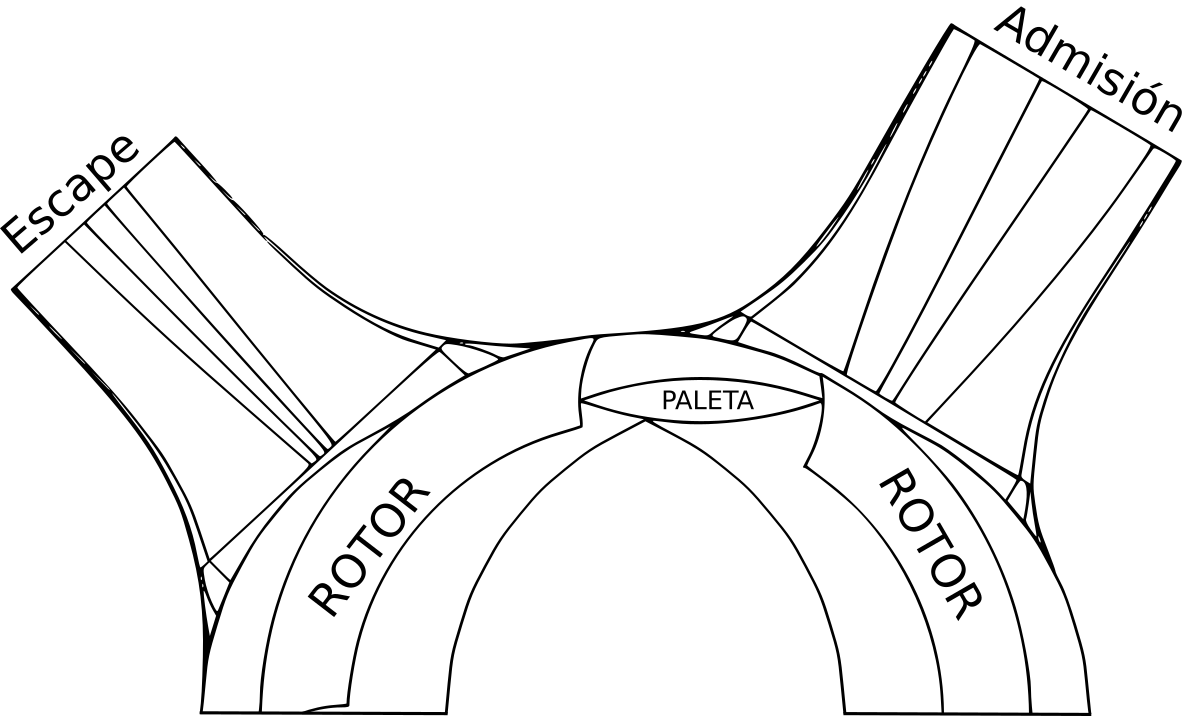
\includegraphics[width=0.7\textwidth]{primer_iteracion.png}
  \caption{Primer Iteración - Modelo CAD}
  \label{fig:primer_it}
\end{figure}
